% Capítulo 2
\chapter{Referencial Teórico} \label{cap:referencial_teorico}

\section{Controle de frequência} \label{sec:controle_freq}

Nos sistemas modernos o controle sobre a frequência do processador pode ser feita por hardware com circuitos independentes como também por software. Para isso existe o Advanced Configuration and Power Interface \abrv[ACPI -- Advanced Configuration and Power Interface]{(ACPI)} um padrão aberto adotado por sistemas operacionais para configurar componentes de hardware relacionados a gerenciamento de energia.

No ACPI são definidos dois estados importantes para o DVFS que otimizam o consumo de energia. São eles o "C", que é ativado quando o processador não está executando nenhuma instrução, e o "P", ativado enquanto o processador está operando. Esses estados possuem diversos níveis e em cada nível a frequência e tensão são alterados.

O estado P começa no nível P0, onde a frequência e tensão são as máximas possíveis, depois o P1, onde diminui ambos, até chegar no último estado, Pn, onde a frequência e tensão são as menores possíveis. A mudança de estado depende do nível de utilização do processador. Para se manter em cada estado, o nível de utilização do processador deve está dentro de limites específicos. Apos ultrapassar esses limites por um determinado tempo, o estado irá mudar para o próximo estado correspondente a esse novo nível de utilização do processador. O número de estados possíveis depende de cada fabricante.

Após um tempo ocioso, o processador começa a ativar os estados C, começando pelo C0 onde ele ainda está completamente ativo, depois passando para o C1, onde alguns recursos são desabilitados, até o Cn, em que todos os recursos possíveis são desabilitados. No padrão ACPI são estabelecidas as funcionalidades que podem ser desabilitadas entre o nivel C1 e o nível C3, como vistas na Tabela \ref{tab:estados_c}. Os demais níveis são específicos de cada fabricante. 

\begin{table}[H]
	\centering
	\begin{tabular}{|l|l|l|}
		\hline
		Modo & Nome            & Funcionalidade                \\ \hline
		C0   & operating state & Processador ativo             \\ \hline
		C1   & Halt            & Para de executar instruções   \\ \hline
		C2   & Stop-Clock      & Desabilita o clock interno    \\ \hline
		C3   & Sleep           & Desabilita coerência de cache \\ \hline
	\end{tabular}
	\caption{Estados C}
	\label{tab:estados_c}
\end{table}

No estado C, quanto maior o nível maior é a economia de energia, porém o retorno ao nível totalmente funcional é mais difícil. Já nos estados P, existe troca entre desempenho e economia de energia. A Figura \ref{fig:p_state} ilustra melhor a troca de estados, nela podemos ver quais partes dos circuitos são desativadas nos estados C, a latência para voltar a o estado ativo, o consumo de potência e também mostra a relação dos estados P com a frequência.

\begin{figure}[H]
	\centering
	\begin{subfigure}[t]{0.5\textwidth}
		\centering
		\includegraphics[height=7.5cm]{Imagens/C-states.png}
		\caption{Estados C}
	\end{subfigure}%
	~ 
	\begin{subfigure}[t]{0.5\textwidth}
		\centering
		\includegraphics[height=7.5cm]{Imagens/P-states.jpg}
		\caption{Estados P}
	\end{subfigure}	
	\caption{Ilustração dos estados C e P}{Imagem alterada de \protect\url{https://www.thomas-krenn.com/en/wiki/Processor_P-states_and_C-states}}
	\label{fig:p_state}
\end{figure}


%Os estados C e P são ortogonais, eles operam de forma independente?

Para esse gerenciamento, o sistema operacional disponibiliza no espaço de usuário uma forma de controlar a frequência. Neste trabalho foi utilizado um sistema operacional que tem como núcleo o Linux.

O Linux é compatível com diversas arquiteturas modernas e amplamente utilizado em servidores, smartphones e supercomputadores. Ele foi baseado no sistema UNIX que tem como filosofia tratar tudo no sistema como um arquivo, incluindo configurações e dispositivos de entrada e saída, como teclado, mouse e disco rígido. Outra característica importante é que ele é modular e partes do sistema podem ser carregadas ou removidas durante sua execução.

No Linux existem diversas opções de gerenciamento de frequência \cite{Brown2005}. Os principais são o acpi-cpufreq, Intel P-state, AMD powernow. Neste trabalho foi utilizado o acpi-cpufreq que é padrão e permite o controle direto da frequência através dos arquivos de sistema. O acpi-cpufreq é um módulo do Linux que utiliza de políticas implementadas que decidem dinamicamente a frequência a ser utilizada. Algumas dessas politicas são:

\begin{itemize}
\item Performance - configurado para a maior frequência possível
\item Powersave - configurado para a menor frequência possível
\item Userspace - o usuário escolhe a frequência a ser utilizada 
\item Ondemand -  controla a frequência dependendo da carga do processador. Quando a carga aumenta a frequência também aumenta de acordo.
\item Conservative - semelhante ao Ondemand mas de forma mais suave, o incremento da frequência é continuo ao invés de ser em saltos.
\end{itemize}

\section{Monitoramento do consumo de potência} \label{sec:monitoramento}
Para medir a potência consumida foram utilizadas as interfaces Running Average Power Limit \abrv[RAPL -- Running Average Power Limit]{(RAPL)} e Intelligent Platform Management Interface \abrv[IPMI -- Intelligent Platform Management Interface]{(IPMI)} descritas em \cite{November2013}.

\subsection{IPMI}
IPMI \cite{November2013} é um conjunto de especificações para subsistemas autônomos que fornece gerenciamento e monitoramento independente de processador, firmware e sistema operacional. A utilização do IPMI permite que os administradores de sistema não precisem se deslocar até o local do servidor, que muitas vezes é distante, para realizar suas tarefas. Também, servidores ficam em locais com baixa temperatura e com muito ruído sonoro devido ao sistema de ventilação, e deve-se evitar passar muito tempo nesses locais. Com o gerenciamento remoto é possível ligar e desligar o sistema, acessar remotamente a \abrv[BIOS -- Basic Input Output System]{(BIOS)} e reinstalar o sistema em caso de alguma falha grave.

\begin{figure}[H]
\centering
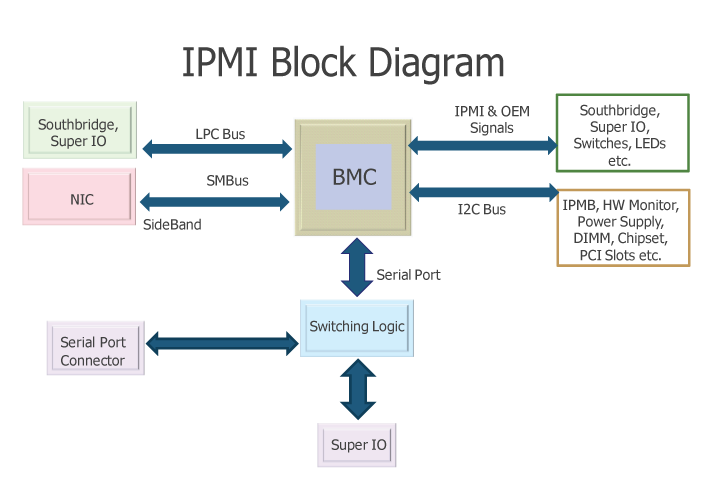
\includegraphics[height=7.5cm]{Imagens/IPMI-Block-Diagram.png}
\caption{Diagrama do IMPI}{Imagem retirada de \protect\url{https://pt.wikipedia.org/wiki/Intelligent_Platform_Management_Interface}, são mostrado os principais componentes do IPMI e como eles se comunicam}
\label{fig:IPMI}
\end{figure}

O  acesso a rede do IPMI pode ser feito pelo protocolo HTTP ou por uma ferramenta disponibilizada pelo fabricante (ipmitool), que também realiza o acesso via rede. Ele também é utilizado para monitorar o status da plataforma com um conjunto de sensores acoplados como temperaturas do sistema, tensões, ventiladores e fontes de alimentação.

\subsection{RAPL}

Microprocessadores Intel modernos, a partir da arquitetura SandyBridge, incluem a interface RAPL \cite{Rotem2012, Hahnel2012, Hackenberg2015} projetada para limitar o uso de energia em um chip ao mesmo tempo que garante o máximo desempenho. Essa interface suporta recursos de medição de energia através de um circuito integrado que estima o uso de energia com base em um modelo conduzido por contadores de eventos arquiteturais de todos os componentes. Além disso também fornece leituras de temperatura e modelos de vazamento de corrente. As estimativas são disponibilizadas em registradores específico de modelo \abrv[MSR -- Model Specific Register]{(MSR)}, sendo atualizado na ordem de milissegundos. As estimativas de energia oferecidas pela RAPL foram validadas pela Intel que mostrou ótimos resultados.